\section{Experiments} \label{sec:result}
We take four applications including Matrix Multiplication (MM), 
FIR, Kmean(KM) and Sobel Edge Detector (SE) as our benchmark. 
The benchmark configurations are presented in table \tabref{tab:benchmark-config}.

\begin{table}[H]
  \caption{Benchmark Configurations \label{tab:benchmark-config}}{
  \centering
  \begin{tabular}{l|l|l}
  \hline
  Benchmark & Parameters & Loop Structure \\ \hline
  MM & Matrix Size(128) & $128 \times 128 \times 128$ \\ \hline
  FIR & \tabincell{l}{\# of Input (1024) \\ \# of Taps+1 (64)} & $1024 \times 64$ \\ \hline
  SE & \tabincell{l}{ \# of Vertical Pixels (128) \\ \# of Horizontal Pixels (8)} & $128 \times 8 \times 3 \times 3$ \\ \hline 
  KM & \tabincell{l}{\# of Nodes(1024) \\ \# of Centroids(4) \\ \# of Dimensions(2)} & $1024 \times 4 \times 2$ \\ \hline  
  \end{tabular}
  }
\end{table}

The benchmark is customized to a CPU-FPGA system using both the proposed 
revenue aware (RA) customization framework and an exhaustive search(ES) based customization. 
Then the customization speed and quality of the two are compared. 

\subsection{Experiment Setup}
All the run time was obtained from a computer with Intel(R) Core(TM) 
i5-3230M CPU and 8GB RAM. Zedboard which has an ARM processor and 
an FPGA was used as the hybrid computation system. Vivado 2013.3 was 
used for the hardware design. 

The overlay typically runs at 200MHz on Zedboard and we 
assume the implementation frequency can be scalable to all the 
different overlay configurations. The power used in this work is 
acquired from XPower which is part of the Vivado design suite.

There are many different design parameters for compiling a nested 
loop to the CPU-FPGA system through an SCGRA overlay. 
\tabref{tab:designparameter} is a list of the major design 
parameters of the overlay customization for nested loop acceleration. 
As identified in the table, most of the parameters are covered in this work 
while pipeline depth, SCGRA topology and operation set of the overlay are not 
configurable at the moment. We adopt a deterministic 200MHz pipeline design 
and 2D torus topology. The operation set supported by the overlay are mainly simple 
operations with three source operands and a single destination operands.
Also note that IO buffer partition is not fully supported and we can only 
change the IO buffer depth and data width at the moment.

\begin{table}[tb]
\caption{Design Parameters of Overlay Customization For Nested Loop Acceleration\label{tab:designparameter}}{
\begin{tabular}{l|l|l}
\hline
\multicolumn{2}{l|}{Design Parameters} & Is Supported? \\ \hline
\multirow{2}{*}{\tabincell{l}{Nested Loop \\ Compilation}}  & Loop Unrolling Factor & Yes  \\ \cline{2-3} 
                   & Grouping Factor & Yes \\ \hline
\multirow{8}{*}{\tabincell{l}{Overlay \\ Configuration}}  & SCGRA Topology  & No, 2D Torus \\ \cline{2-3} 
                                                          & SCGRA Size  & Yes \\ \cline{2-3}
                                                          & Instruction Mem & Yes \\ \cline{2-3}
                                                          & Data Mem & Yes \\ \cline{2-3}
                                                          & IO Buffer & Yes \\ \cline{2-3}
                                                          & Address Buffer & Yes \\ \cline{2-3}
                                                          & Operation Set & No \\ \cline{2-3}
                   & Pipeline Depth & No \\ \hline
\end{tabular}
}
\end{table}

\subsection{Experiment Results}
\begin{figure}[tb]
	\subfloat[MM]{%
		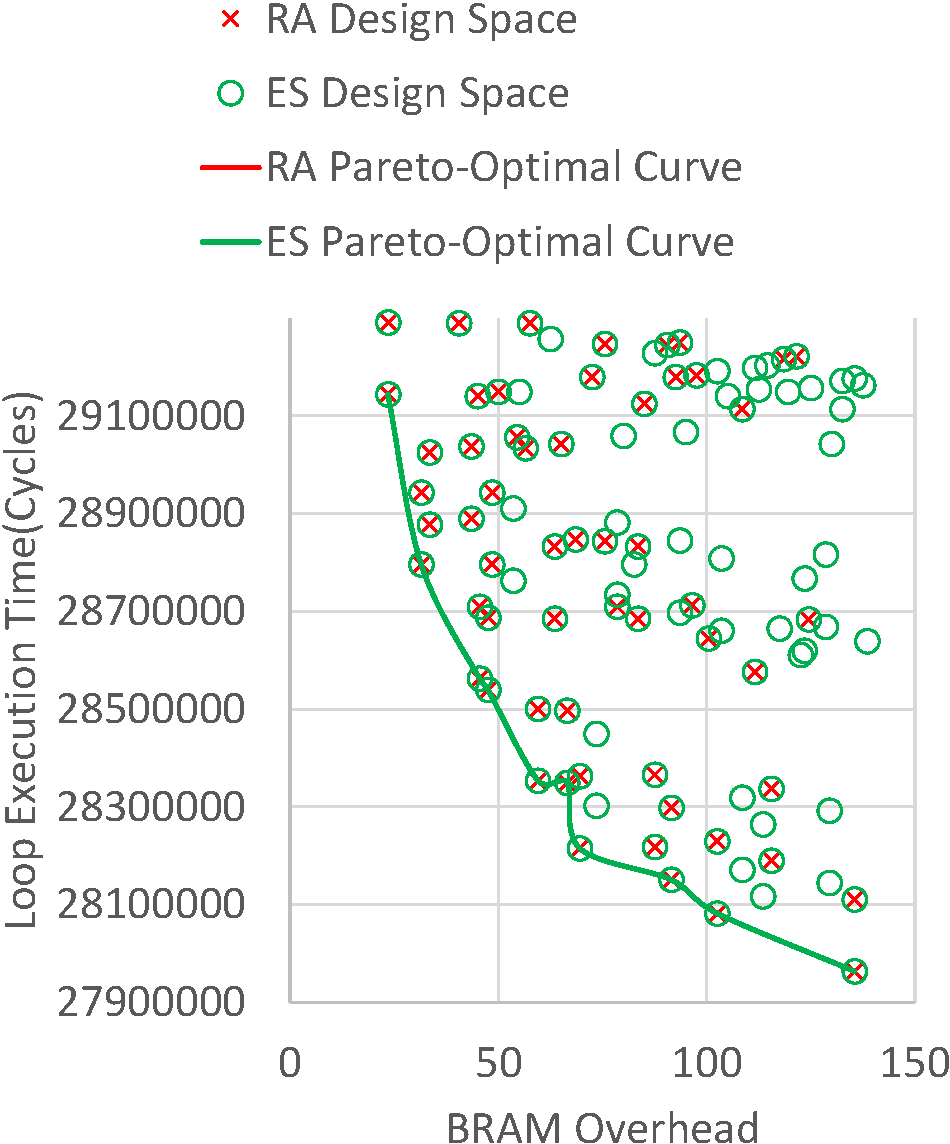
\includegraphics[width=0.21\textwidth]{mm-overhead-perf}
	}
	\subfloat[FIR]{%
		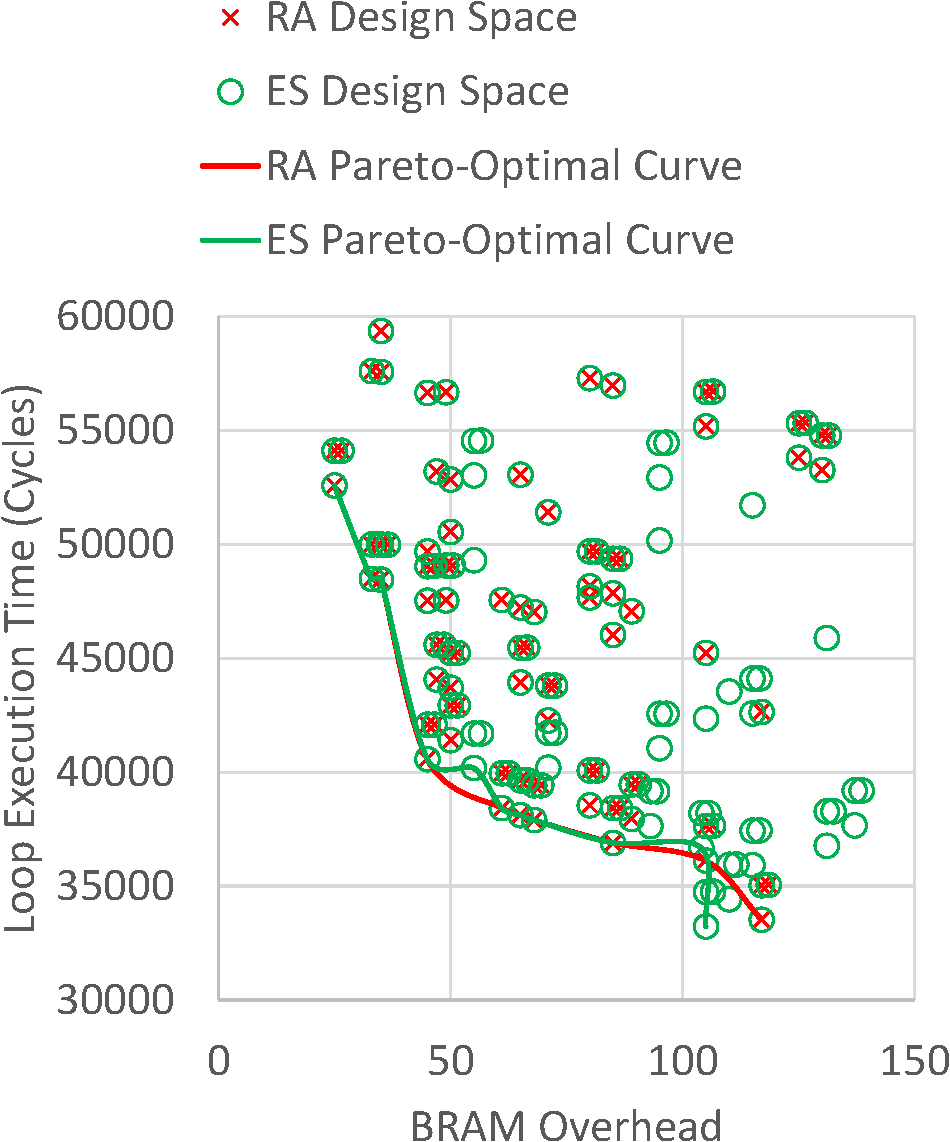
\includegraphics[width=0.21\textwidth]{fir-overhead-perf}
	}
    \hfill
	\subfloat[SE]{%
		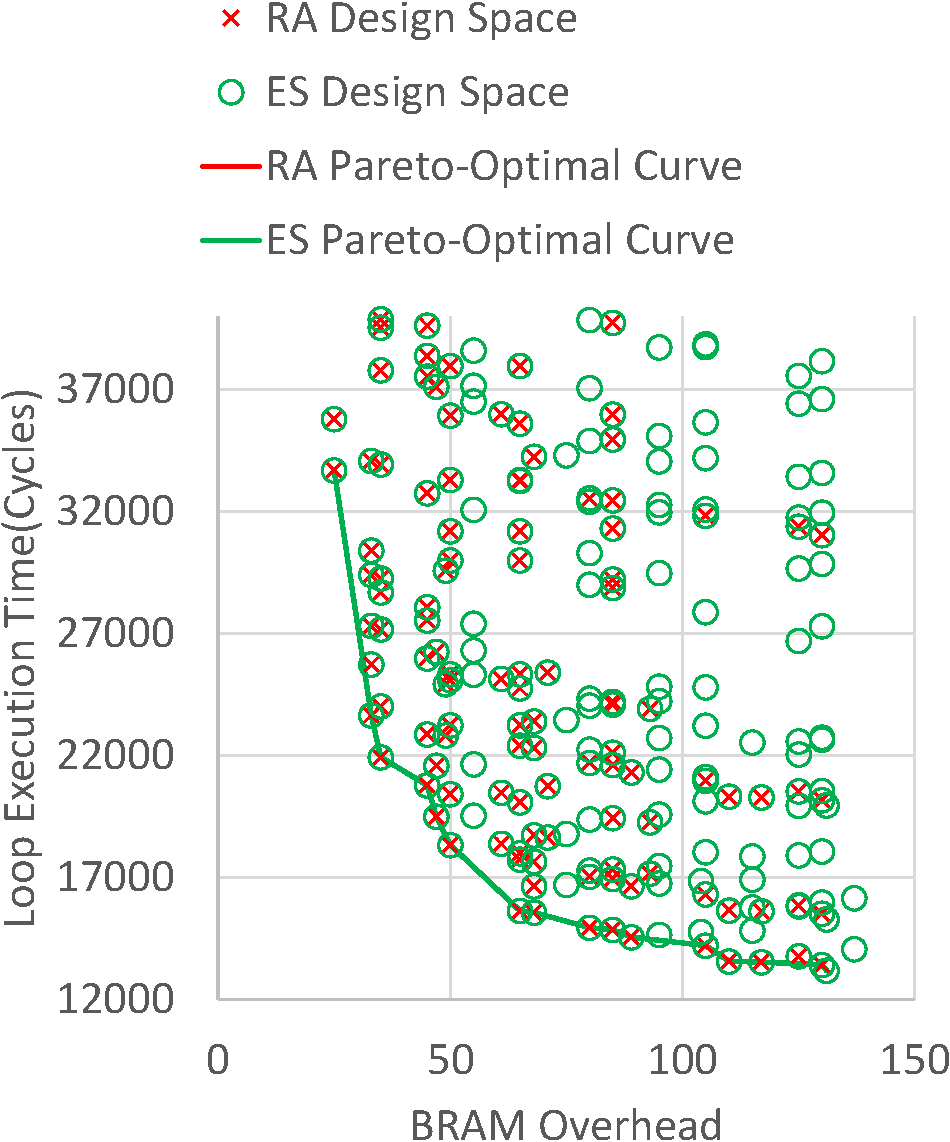
\includegraphics[width=0.21\textwidth]{sobel-overhead-perf}
	}
	\subfloat[KM]{%
		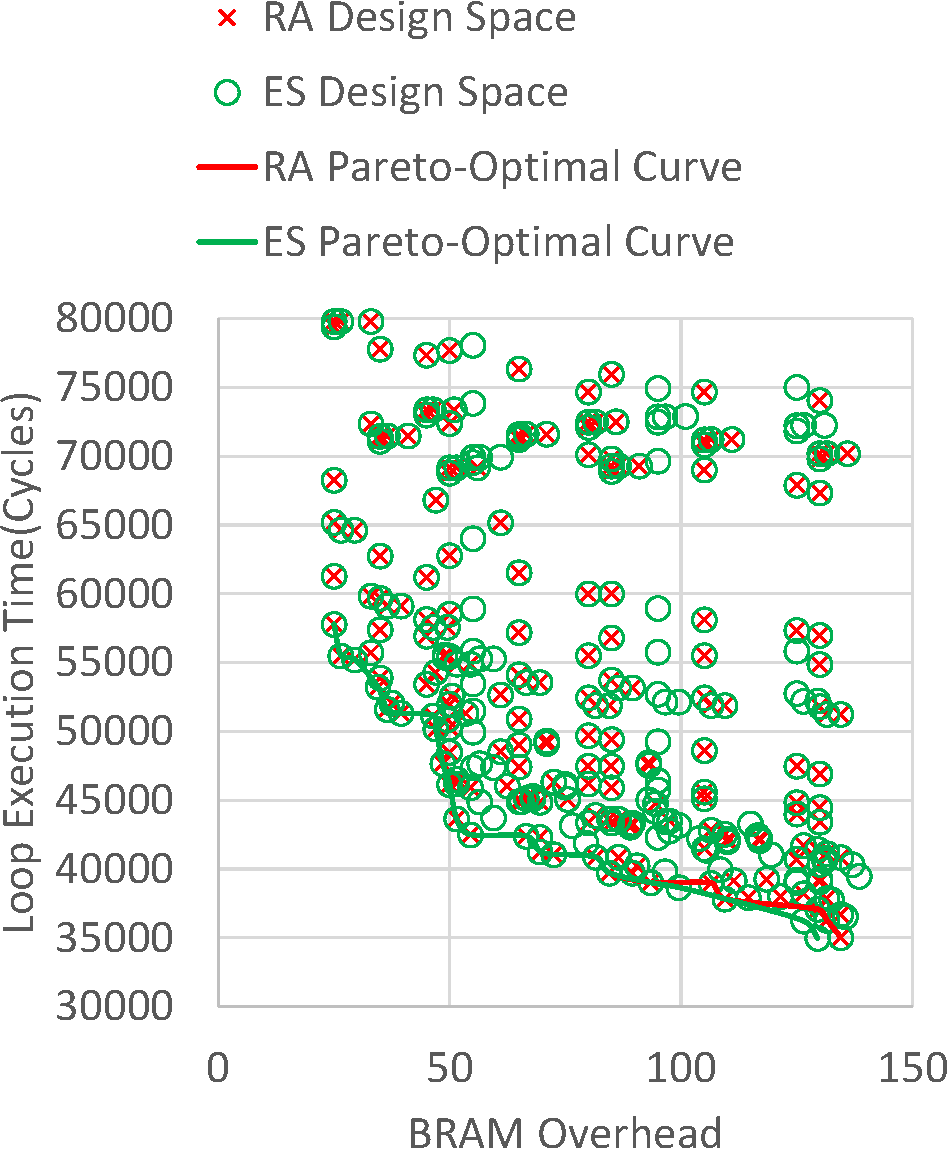
\includegraphics[width=0.21\textwidth]{kmean-overhead-perf}
	}
    \caption{Performance-Overhead Pareto-optimal Curve and Possible Design Options Around The Curve}
	\label{fig:DSE1}
\end{figure}

\begin{figure}[tb]
	\subfloat[MM]{%
		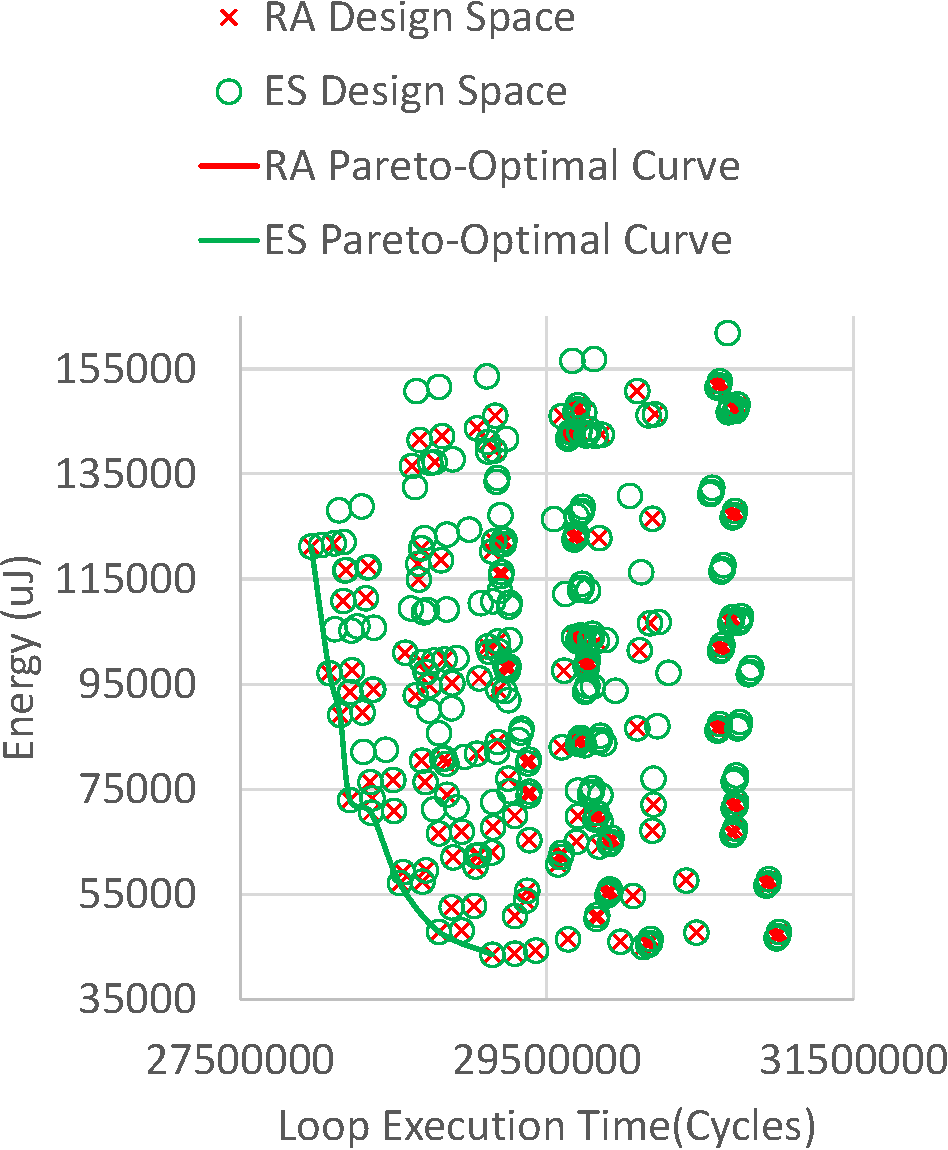
\includegraphics[width=0.23\textwidth]{mm-energy-perf}
	}
	\subfloat[FIR]{%
		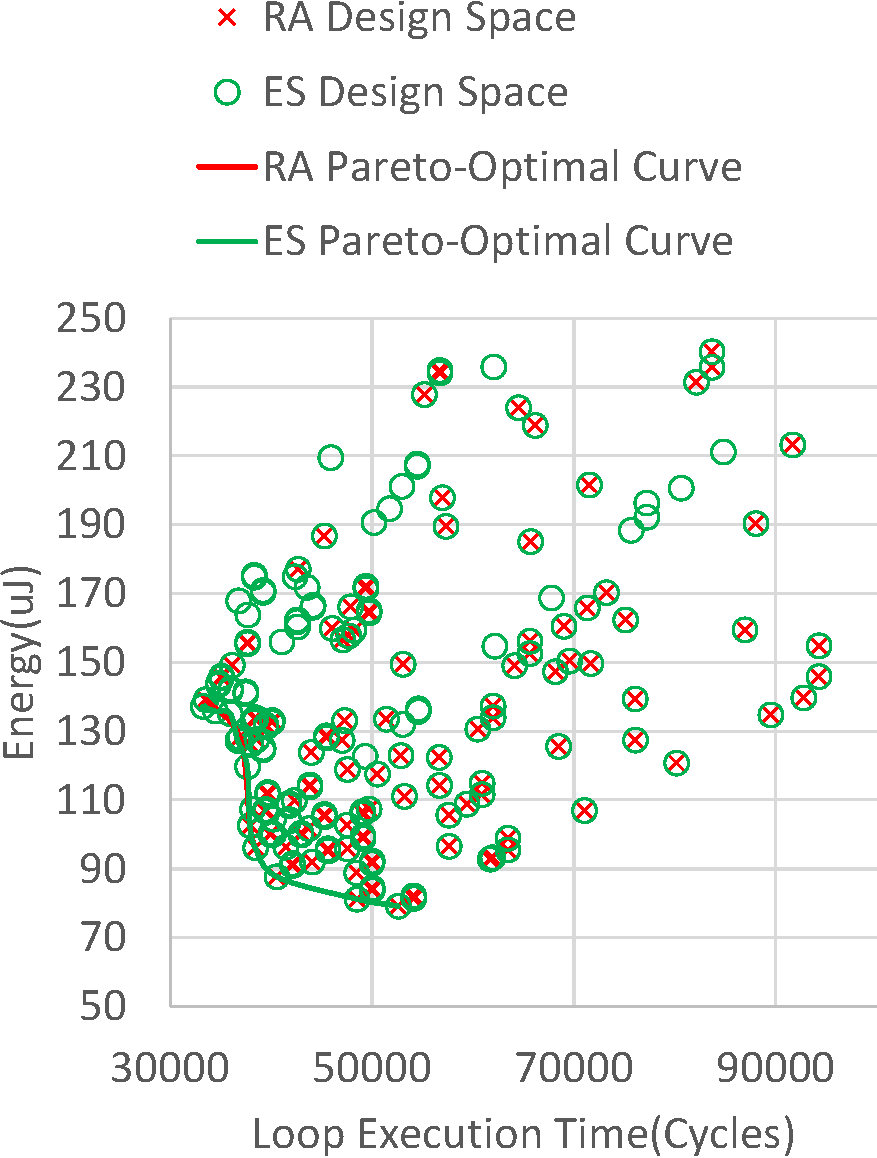
\includegraphics[width=0.21\textwidth]{fir-energy-perf}
	}
    \hfill
	\subfloat[SE]{%
		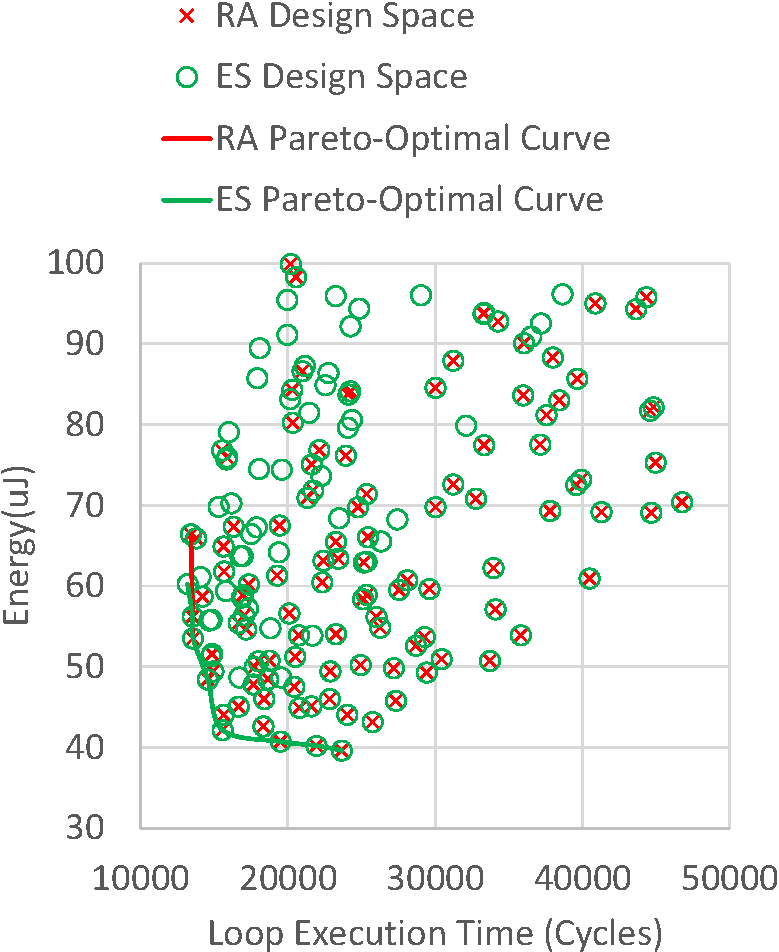
\includegraphics[width=0.21\textwidth]{sobel-energy-perf}
	}
	\subfloat[KM]{%
		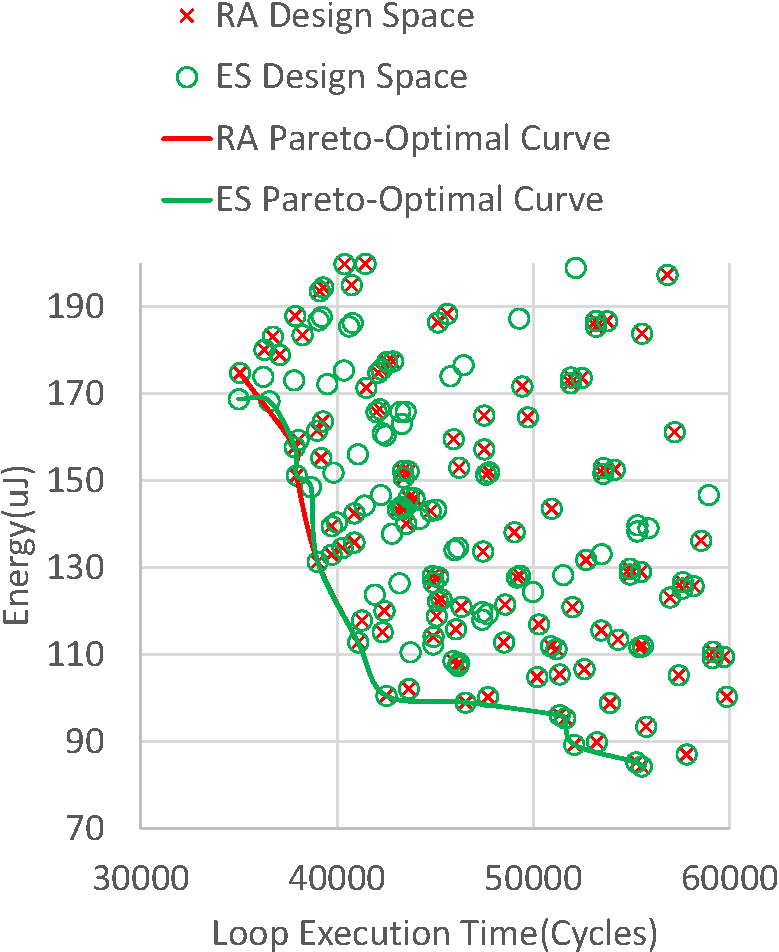
\includegraphics[width=0.21\textwidth]{kmean-energy-perf}
	}
    \caption{Performance-Energy Pareto-optimal Curve and Possible Design Options Around The Curve}
	\label{fig:DSE2}
\end{figure}

\tabref{tab:dsetime} shows the exploration time comparison of the two 
DSE methods. The proposed RA DSE is around 100x faster than the 
ES DSE on average. In particular, it can be found that 
ES DSE can be extremely slow on MM which has three levels of loop with relatively large 
loop count and thus larger design space. Though RA DSE also needs 
longer time to complete the DSE of MM, it can skip most 
of the unfeasible configurations and the run time is less sensitive to the size 
of the design space. 

\begin{table}[tb]
  \caption{Time Cost for RA DSE and ES DSE\label{tab:dsetime}}{
  \centering
  \begin{tabular}{l|l|l|l|l}
  \hline
  Benchmark & MM & FIR & KM & SE \\ \hline
  RA DSE (min) & 20.2 & 10.6 & 13.4 & 11.4\\ \hline
  ES DSE (min) & 2880.6 & 835.2 & 1140.5 & 946.2\\ \hline
  Speedup & 142.6 & 78.8 & 85.1 & 86.2 \\ \hline
  \end{tabular}
  }
\end{table}

In order to demonstrate the quality of RA DSE, we presented the comparison 
of the exploration results acquired from both DSE methods. The exploration results 
includes performance-overhead, performance-energy and performance-EDP trade-offs 
as shown in \figref{fig:DSE1}, \figref{fig:DSE2} and \figref{fig:DSE3} respectively.
In the figures, both Pareto-optimal curves and the design options around the curves are 
presented. 

Basically, the Pareto-optimal curves acquired using RA DSE is quite close to that 
obtained from an ES DSE. In particular, all the three Pareto-optimal curves of MM are highly 
overlapped and RA DSE successfully skips the design options that are further from the Pareto-optimal 
curves. However, RA DSE may prune the design options that involve a larger 
overlay size but better performance according to the revenue 
metric. As a result, the Pareto-optimal curves of the rest three 
nested loops mostly deviate at the higher performance area. Fortunately, this can be improved by 
lowering the performance revenue threshold and affording longer DSE time.

These Pareto-optimal curves can also be used for customization. When minimum energy 
consumption or minimum EDP is taken as the design goal, RA aware DSE can achieve the 
optimal design in all the four benchmarks. 

\begin{figure}[tb]
	\subfloat[MM]{%
		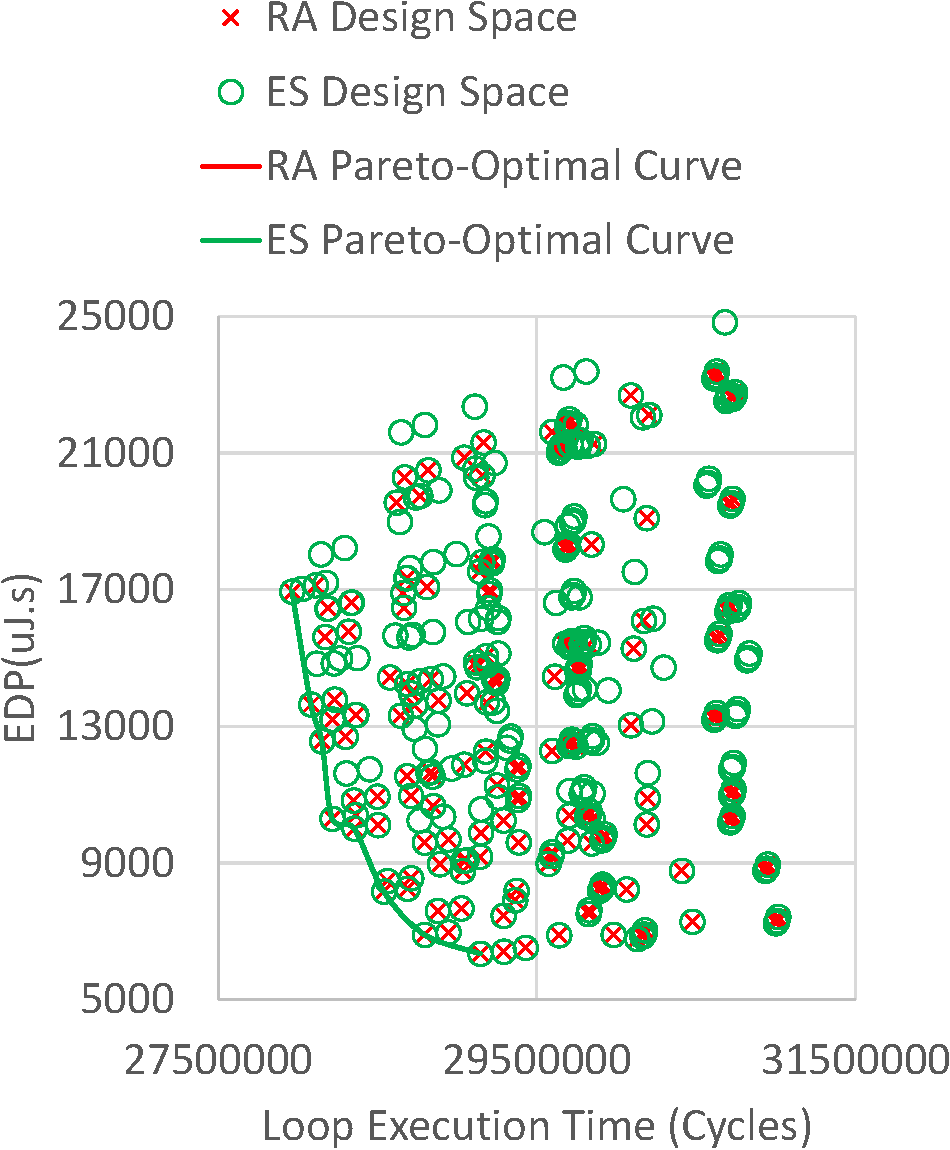
\includegraphics[width=0.23\textwidth]{mm-EDP-perf}
	}
	\subfloat[FIR]{%
		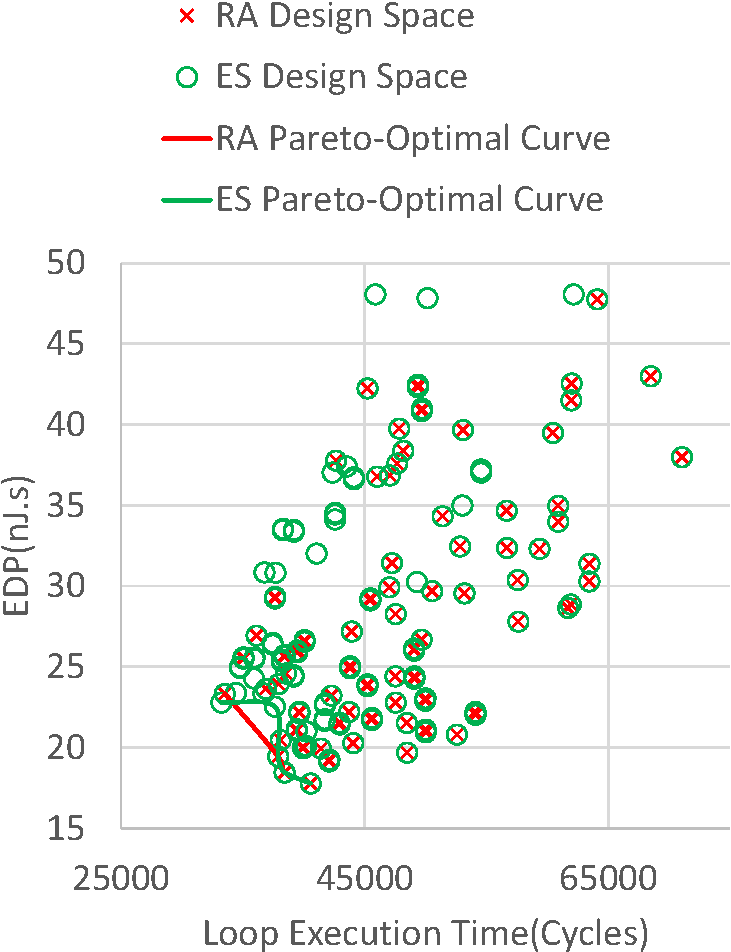
\includegraphics[width=0.21\textwidth]{fir-EDP-perf}
	}
    \hfill
	\subfloat[SE]{%
		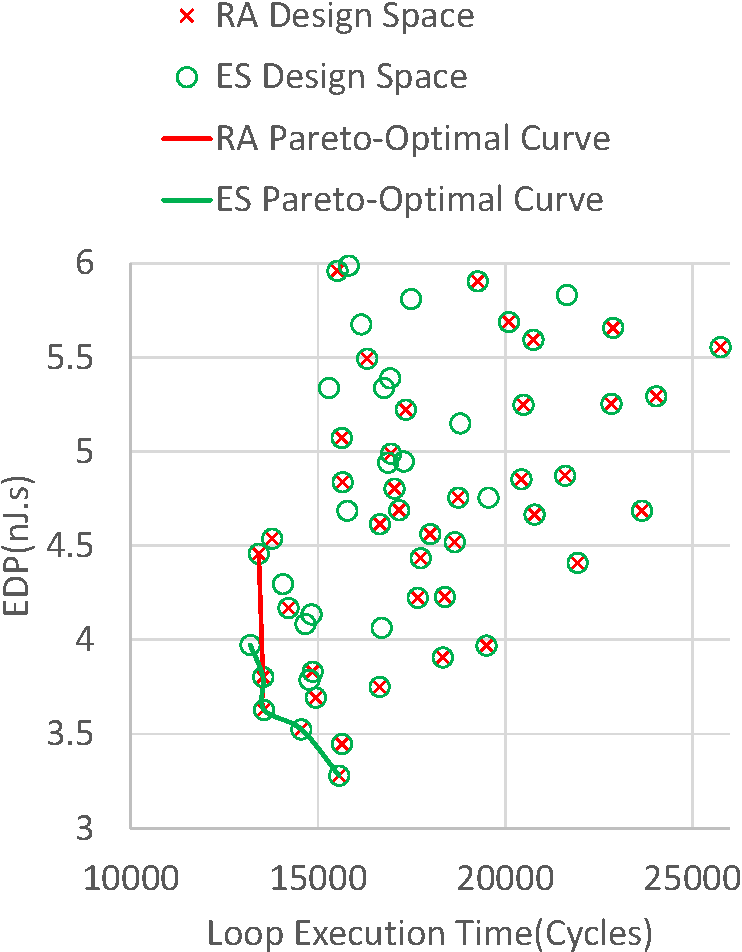
\includegraphics[width=0.21\textwidth]{sobel-EDP-perf}
	}
	\subfloat[KM]{%
		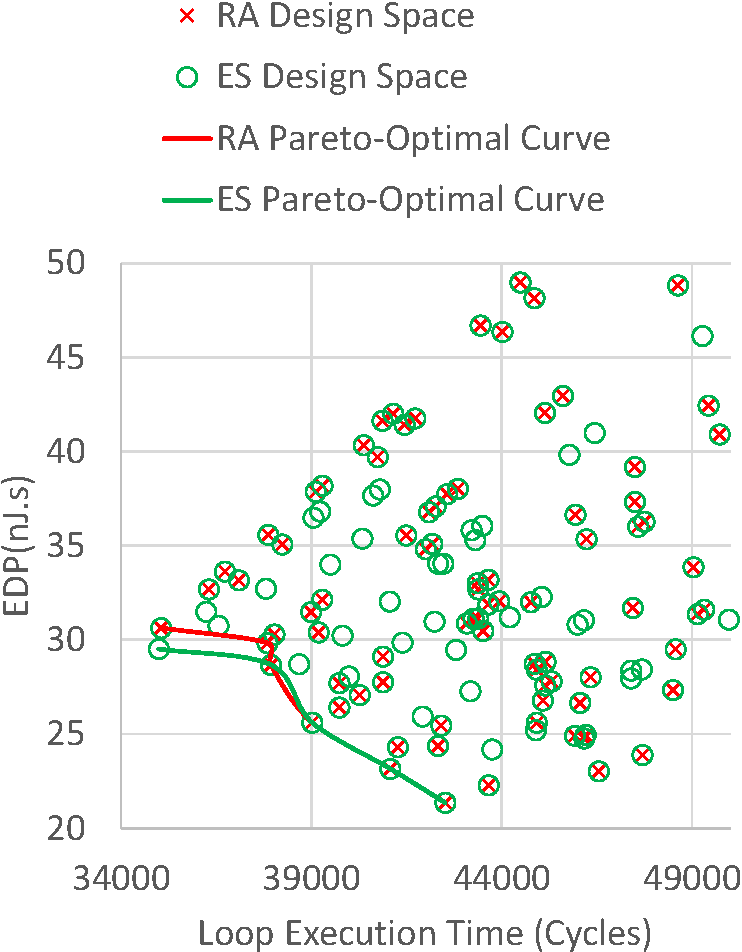
\includegraphics[width=0.21\textwidth]{kmean-EDP-perf}
	}
    \caption{Performance-EDP Pareto-optimal Curve and Possible Design Options Around The Curve}
	\label{fig:DSE3}
\end{figure}


